\chapter{Réalisation technique}

\subsection{Descriptif général}

Nous avons fait le choix de déployer des clusters
Kubernetes\footnote{\url{https://kubernetes.io/fr/}}
pour un certain nombre de raisons. Tout d'abord, Kubernetes est une
technologie répandue et approuvée à très grande échelle, ce qui en fait
une référence incontournable en termes de fiabilité pour architecturer
une infrastructure devant répondre à un certain nombre de problématiques
bien précises, telles que la redondance, la tolérance aux pannes et à la
charge, etc\.
Ce qui correspond à la demande de nos clients.

En outre, découper notre projet en micro-services nous a permis de
découper les tâches de manière plus fines et d'avancer parallèlement sur
ces derniers. Chaque service est testé et compilé avant d'être
conteneurisé automatiquement sous forme de conteneur
Docker\footnote{\url{https://www.docker.com/}}. Ces
derniers peuvent ainsi être déployés très facilement sur une
infrastructure Kubernetes pour la grande instance de production, ainsi
que sur une instance minimaliste avec l'aide de
\textit{docker-compose}\footnote{\url{https://docs.docker.com/compose/}},
qui va simplement lancer une instance de chaque service. Cette dernière
solution est pratique à la fois pour les développeurs pour faire tourner
l'ensemble de l'application en local chez eux, ainsi que pour nos
clients qui auront la possibilité de lancer une nouvelle instance
minimaliste lors de leurs déplacements alors qu'ils n'ont pas de
connexion à leur serveur principal pour continuer à communiquer.

Nous avons également choisi de faire des micro-services car notre
application était supposée être modulaire. Nous n'avons pas retravaillé
cette partie de l'architecture logicielle lorsque nous avons abandonné
cet objectif, car il aurait été trop long de tout redévelopper..

Les machines virtuelles que nous avons ont été configurées avec l'aide
d'Ansible\footnote{\url{https://www.ansible.com/}}, de
même que la base des clusters Kubernetes avec l'aide de
\textit{Kubespray}\footnote{\url{https://kubespray.io/\#/}}, un
Playbook Ansible, ce qui nous permet d'avoir un déploiement automatisé
assez rapide. Un nouveau cluster complet peut être monté en une heure
environ.

\subsection{Gestion de flux de données très importants}

L'utilisation de Kubernetes ainsi que la pile de surveillance que nous
avons mis en place nous permettent de récupérer un certain nombre de
métriques. Le fait d'avoir architecturé notre application sous forme de
micro-services nous permet de monter ou diminuer le nombre d'instances
d'un de ces services de manière indépendante avec l'aide des métriques
que nous avons récupérés, ce qui permet d'adapter les ressources de nos
clusters en fonction de la demande courante, et donc de pouvoir
s'adapter à des flux de données très importants peu importe le service
sollicité.

De plus, le bus de données permet d'éviter aux services d'avoir à gérer
la notion de charge. En effet, c'est le bus de données qui temporise
l'ensemble des requêtes en attente avec l'aide de \textit{Nats-Streaming
(aka. stan)}\footnote{\url{https://docs.nats.io/nats-streaming-concepts/intro}}

\subsection{Tolérance aux pannes}

Nous avons deux clusters Kubernetes répartis sur deux sites
géographiquement distincts : l'un à Illkirch et l'autre à Esplanade. Si
l'un des deux venait à tomber, l'autre sera là pour prendre la charge et
répondre à la demande.

Nos clusters Kubernetes sont chacun constitués de trois nœuds,
permettant de mutualiser l'ensemble des ressources au sein du cluster.
Si au sein d'un cluster on perd un nœud, il en restera toujours deux qui
seraient disponibles, soit la majorité ; Kubernetes peut donc continuer
à instancier de nouvelles instances sans difficultés. Par contre si on
venait à perdre un second nœud au sein de ce cluster, il n'y aurait plus
la majorité. Les services actuellement en place sur le dernier nœud
resteront accessibles, mais les services se trouvant sur les autres
nœuds ne pourront pas être déployés sur ce dernier nœud comme cela
pourrait être le cas dans le cas précédent.

Chaque cluster expose l'application depuis une adresse IP qui est
assignée à l'un des nœud. Si le nœud en question venait à tomber, cette
adresse IP sera attribuée à un autre nœud du cluster qui est disponible.
Ce point sera davantage détaillé dans la suite de ce mémoire.

En termes de maintenance, remplacer un service, par exemple dans le
cadre d'une mise à jour, est invisible pour l'utilisateur final, car
Kubernetes va d'abord instancier la nouvelle instance du micro-service
et va arrêter l'ancienne seulement une fois que la nouvelle instance
sera fonctionnelle ; c'est-à-dire que si une nouvelle instance n'arrive
pas à se lancer correctement, l'ancienne instance, qui elle est
fonctionnelle, continuera à répondre aux différentes demandes. De plus,
il est possible d'avoir plusieurs instances d'un même service au sein
d'un cluster pour avoir de la redondance et mieux résister aux pannes,
ainsi que pour mieux gérer la charge.

Au niveau de l'application web, si la connexion au WebSocket plante, la
connexion va se rétablir automatiquement ultérieurement, et ce de
manière périodique toutes les deux secondes jusqu'à ce que la connexion
s'effectue à nouveau (le temps que le serveur soit à nouveau accessible
en cas d'une panne de forte envergure par exemple).

Du côté de la base de données, étant donné que l'on déploie des clusters
de PostgreSQL avec Stolon que l'on verra plus tard dans ce mémoire, nous
avons une redondance qui évite une perte de données. De plus ces données
sont persistés sur le disque contrairement aux autres données qui n'ont
pas besoin de persistance. Le site d'Esplanade héberge notre cluster
Postgres maître. S'il tombe, alors seuls les lectures pourront être
possibles ce qui constitue un mode dégradé. Il en va de même avec notre
bus de donné, qui est fédéré entre les deux sites, avec une instance
maître sur Esplanade.

\subsection{Tolérance à la charge, redimensionnement automatique}

Comme dit dans la partie précédente, il est possible d'avoir plusieurs
instances d'un même service qui sont lancés au sein d'un même cluster.
Il est possible de mettre en place des règles afin que ces derniers
soient par exemple lancés de préférence sur des nœuds différents. C'est
par exemple le cas du contrôleur d'\textit{ingress} qui a une instance
lancée par nœud.

Il est également possible de changer le nombre d'instances d'un service
en fonction de certaines métriques, notamment les ressources utilisées
telles que la RAM et le CPU, ou bien des métriques personnalisées
récupérées par notre pile de surveillance en explorant des URL précises
exposées par les services.

Si jamais notre application deviendrait très populaire, il serait
toujours possible de rajouter de nouvelles machines au sein des clusters
existants, voire même ajouter des clusters entiers.

\subsection{Temps de réponse garantis}

Nous ne garantissons pas spécialement de temps de réponse pour notre
application. Néanmoins le fait qu'elle supporte bien la charge et que
l'on peut faire évoluer le nombre d'instances des différents services en
fonction de certaines métriques, on peut limiter le temps d'attente pour
le traitement des différentes requêtes en cas de montée en charge.

Le fait d'avoir une tolérance aux pannes plutôt convenable nous aide
également à limiter les temps de réponses : puisque les requêtes ont
moins de chances d'échouer, il y aura moins de tentatives à effectuer
avant d'accéder aux différentes ressources.

\subsection{Hébergement sur deux sites}

Nous n'avions aucune ressource à disposition, ni matérielles, ni
financières pour être en mesure de répondre à la demande, excepté les
machines en salles de TP\.
L'utilisation de ces dernières n'étaient malheureusement pas envisageables
dans le cadre de ce projet étant donné que ces machines sont utilisées lors
de différents TP et qu'il faudrait par conséquent réinstaller toute
l'infrastructure à séance de travail fois avoir un environnement maîtrisé.

Ludovic est donc allé voir différentes personnes au sein de l'Université
afin de voir s'il était possible de venir avec son propre serveur 1U ou
s'il était possible d'obtenir des machines virtuelles quelque part.
Déployer un nouveau serveur au sein de l'Université est malheureusement
trop complexe. Il a finalement pu trouver des machines virtuelles pour
l'ensemble des groupes de projet à Illkirch ; c'est ainsi que nous
avions eu nos quatre première machines virtuelles pour y déployer notre
premier cluster Kubernetes.

Le premier cluster situé à Illkirch est constitué de trois machines
virtuelles (\texttt{chatalk-balzac}, \texttt{chatalk-camus} et
\texttt{chatalk-zola}) qui sont configurés pour être les trois nœuds
maîtres de ce cluster. Ces machines virtuelles sont dotés de 8vCPU,
de 8Go de RAM, de 50Go de disque et ont pour système d'exploitation
Ubuntu Server 18.04, qui correspond à la dernière LTS.

Une quatrième machine virtuelle (chatalk-dumas) est déployée sur ce site
pour des fins utilitaires. Elle dispose des mêmes ressources que les
trois autres machines virtuelles, sauf en termes de disque où il y a
75Go à sa disposition. Cette machine virtuelle est utilisée pour y
héberger Minio (s3), qui est un stockage compatible S3, un type stockage
qui a la possibilité de passer à l'échelle de manière plus efficace que
les solutions classiques à base de montages distants. Ce stockage est
utilisé pour héberger nos sauvegardes ainsi que ce qu'il faut pour
initialiser une nouvelle instance de la base de données. Cette machine
virtuelle est également utilisée pour héberger des exécuteurs
\textit{GitLab} qui nous permettent de tester, compiler et déployer notre
application très rapidement en production. Cette machine virtuelle nous
sert également pour héberger nos propres images Docker dans notre base
de registre (\textit{registry}).

Ludovic a pu obtenir dans un second temps quatre autres machines
virtuelles à Esplanade pour former un second site. Les machines
virtuelles chatalk1, chatalk2 et chatalk3 sont les trois nœuds utilisés
pour le second cluster Kubernetes, qui ont les mêmes ressources que le
premier cluster. La dernière machine virtuelle, chatalk4, n'a pas été
utilisée pour le moment. Elle aurait pu nous permettre de redonder le
stockage s3 par exemple, et par conséquence de s'assurer qu'il soit
toujours accessible même si le site d'Illkirch venait à tomber ; hélas
par manque de temps nous n'avons pas pu le faire.

Nous avons donc réussi à avoir toutes nos ressources au sein de
l'Université de Strasbourg, et ce sur deux sites différents
géographiquement (Illkirch et Esplanade), même si cela n'a pas forcément
été très simple de les avoir. De surcroît, chaque demande (demande
d'ouverture de ports, augmentation des ressources, demande d'IP
publiques, \ldots) devait être faite par mail ou en personne, une partie
d'entre elles étant remontées jusqu'au support informatique de
l'Université, ce qui peut prendre du temps. Il n'était donc pas possible
de faire des tests très poussés concernant l'extinction de machines
virtuelles. En effet, il aurait fallu attendre que quelqu'un nous les
rallume. Enfin, accéder aux machines virtuelles nécessite de passer par
le réseau de l'Université, ce qui oblige à passer par une connexion VPN
si l'on souhaite travailler à distance. L'université n'a également pas
été en mesure de nous fournir de l'IPv6 pour nos différentes machines
virtuelles.

Le schéma suivant illustre l'architecture actuelle de notre projet :

\begin{figure}
  \caption{\label{infra-arch} Architecture de l'infrastructure de ChaTalK}
  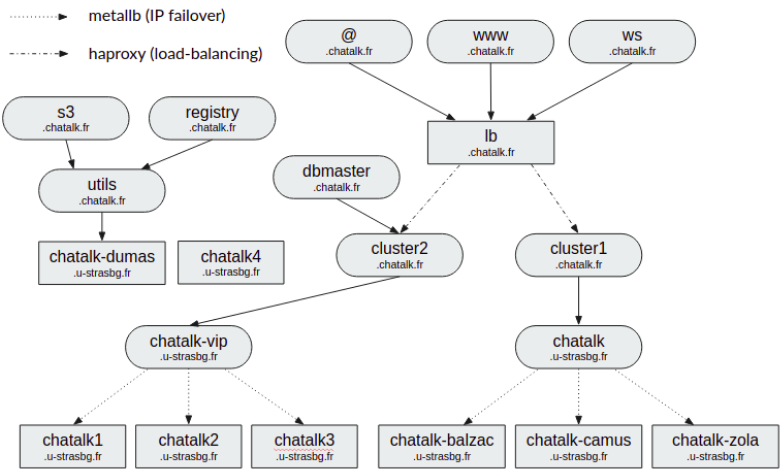
\includegraphics[width=15cm]{images/infra-arch}
\end{figure}

Chaque cluster Kubernetes fait tourner les éléments suivants :

\begin{itemize}
\item
  un contrôleur d'entrée (nous utilisons
  \textit{nginx-ingress-controller}\footnote{
    \url{https://kubernetes.github.io/ingress-nginx/}}
  qui est celui pris officiellement en charge par Kubernetes), qui
  permet de rediriger le trafic entrant vers les bons services hébergés
  sur le cluster,
\item
  une solution de basculement d'IP avec l'aide du projet
  \textit{metallb}\footnote{
    \url{https://metallb.universe.tf/concepts/layer2/}}
  ; en demandant une IP supplémentaire pour chaque cluster
  (\textit{chatalk} pour cluster1 et \textit{chatalk-vip} pour cluster2)
  metallb va l'attribuer à l'un des nœuds du cluster. Si un des nœuds du
  cluster en question tombe, cette IP sera automatiquement attribuée à
  un autre nœud qui est disponible si c'était ce nœud qui possédait
  cette adresse. Le fait d'avoir une adresse IP qui est certaine de
  pointer sur un nœud qui est disponible nous permet de faire pointer
  les entrées DNS dessus, le contrôleur d'\textit{ingress} se charge de
  répartir la charge convenablement au sein du cluster. Il s'agit d'un
  mécanisme qui est habituellement déjà en place lorsque l'on est chez
  un fournisseur de services infonuagiques avec l'utilisation de
  \textit{load-balancers} physiques, ce qui n'est pas notre cas.\\
  Metallb est une solution reconnue et est utilisée massivement pour les
  cas similaires au nôtre, c'est la raison pour laquelle nous l'avons
  choisi.\\
  Utiliser de la répartition de charge au niveau DNS n'est pas efficace,
  car si un des trois nœuds d'un cluster tomberait en panne, un tiers
  des requêtes échouerait.\\
  Nous ne pouvons également pas utiliser de l'\textit{anycast} car on
  n'aurait pas la garantie qu'un flux TCP irait sur un même nœud, ce qui
  pourrait s'avérer problématique dans le cas où on récupérerait un gros
  fichier par exemple.
\item
  un bus de données (\textit{nats} /
  \textit{nats-streaming}\footnote{\url{https://nats.io/}}), qui est une
  solution vraiment légère et performante. Apache
  Kafka\footnote{\url{https://kafka.apache.org/}} ou
  RabbitMQ\footnote{\url{https://www.rabbitmq.com/}}
  sont des alternatives qui sont relativement plus grosses, et
  NSQ\footnote{\url{https://nsq.io/}} est une alternative
  similaire à Nats, mais semble être moins utilisé.\\
  Utiliser un bus de données nous permet d'empiler les différents
  messages avec \textit{nats-streaming} en cas de montée en charge
  soudaine, ce qui évite d'avoir à implémenter cette logique dans chacun
  des micro-services.
\item
  un gestionnaire de base de données PostgreSQL
  (\textit{stolon}\footnote{\url{https://github.com/sorintlab/stolon}})
  qui nous permet d'avoir des instances de PostgreSQL en
  haute-disponibilité et de faire de la fédération entre deux sites. Au
  départ nous étions partis sur
  \textit{postgres-operator}\footnote{
    \url{https://github.com/zalando/postgres-operator}}
  de Zalando, mais les logs n'étaient pas assez précis pour permettre de
  déboguer convenablement la solution.
\item
  un ensemble d'outils pour faire de la surveillance, avec l'aide du
  projet \textit{kube-prometheus}\footnote{
    \url{https://github.com/coreos/kube-prometheus}},
  qui nous permet de déployer et configurer assez rapidement
  \textit{AlertManager}\footnote{
    \url{https://prometheus.io/docs/alerting/alertmanager/}},
  \textit{Prometheus}\footnote{\url{https://prometheus.io/}} et
  \textit{Grafana}\footnote{\url{https://grafana.com/}} (voir
  la partie concernant la supervision pour plus d'informations) qui sont
  les outils les plus couramment utilisés pour faire de la supervision
  au sein d'un cluster Kubernetes.
\item
  notre application, que nous allons détailler dans la partie suivante.
\end{itemize}

Afin de rendre notre application accessible en IPv4 et en IPv6 (plus
d'information dans la partie concernant la double-pile), ainsi que pour
faire de la répartition de charge entre les deux sites, Ludovic a mis en
place une machine virtuelle à l'AIUS (lb). Encore une fois, utiliser de
l'\textit{anycast} n'était pas possible, et utiliser de la répartition de
charge au niveau DNS ferait que si l'un des deux sites tombe, la moitié
des requêtes échouerait, ce qui n'est pas envisageable. L'ensemble de
l'infrastructure étant accessible uniquement depuis le réseau de
l'Université, seuls l'interface web et un point d'entrée pour établir
une connexion WebSocket vers l'arrière-plan sont exposés sur Internet
via cette machine virtuelle.

\subsection{Application}

L'application est décomposée en deux grandes parties : la partie
\textit{frontale} qui est l'interface utilisateur, une application web sur
navigateur Internet ou une application mobile sur téléphone, ainsi que
la partie \textit{arrière-plan} qui est l'ensemble des micro-services
déployés pour traiter les différentes requêtes.

\subsubsection{Application web}

Aujourd'hui un site web peut se comporter comme une application
mobile\footnote{
  \url{https://www.howtogeek.com/196087/how-to-add-websites-to-the-home-screen-on-any-smartphone-or-tablet/}}.
De plus, une application web à l'avantage de ne nécessiter qu'un simple
navigateur web moderne à jour et respectant les différents standards ;
pas besoin d'installer quoi que ce soit en plus, ce qui est pratique
pour les utilisateurs, et ce indépendamment de la plateforme utilisée
(ordinateur, télévision, tablette ou smartphone).

L'application web a été développée avec
ReactJS\footnote{\url{https://reactjs.org/}}, une
bibliothèque JavaScript largement reconnue et utilisée, qui permet de
créer une application mobile complète et dynamique en évitant de
réinventer la roue. Nous utilisons
TypeScript\footnote{\url{https://www.typescriptlang.org/}}
qui génère du code JavaScript en offrant l'avantage de faire de la
vérification sur les types, évitant ainsi un grand nombre de bogues en
production.

Cette application web se connecte à l'arrière-plan avec l'aide d'une
connexion WebSocket sécurisée. Un mécanisme de reconnexion au WebSocket
a été mis en place dans le cas où la connexion au WebSocket est
momentanément indisponible ou est interrompue.

\subsubsection{Application mobile}

Ludovic a réalisé une application mobile pour Android avec
Kotlin\footnote{\url{https://kotlinlang.org/}} dans
le cadre de l'UE Programmation Mobile. L'application a été codée en
utilisant les dernières recommandations Android dans l'optique d'avoir
un code propre et maintenable.

L'application a été développée sur Android Studio et a été testée sur
les appareils suivants :

\begin{itemize}
\item
  Pixel 3a, Android Q, API 29 (émulateur d'Android Studio),
\item
  Honor 10, Android P, API 28 (téléphone personnel).
\end{itemize}

Fonctionnalités communes par rapport à l'application web :

\begin{itemize}
\item
  connexion
\item
  inscription
\item
  déconnexion
\item
  lister les conversations
\item
  afficher une conversation
\item
  envoyer un message dans une conversation
\item
  recevoir des messages dans une conversation
\end{itemize}

Fonctionnalités manquantes par manque de temps :

\begin{itemize}
\item
  création d'une nouvelle conversation
\item
  gestion d'une conversation :

  \begin{itemize}
  \item
    ajouter des personnes
  \item
    retirer des personnes
  \item
    renommer une conversation
  \end{itemize}
\item
  respect de la charte graphique\footnote{
    \url{https://blog.chatalk.fr/graphic-charter/}}
\item
  intégration des maquettes\footnote{
    \url{https://blog.chatalk.fr/mock-ups-update/}}
\end{itemize}

Fonctionnalitées supplémentaires :

\begin{itemize}
\item
  Prise en charge du thème sombre : si un utilisateur a configuré son
  appareil Android pour utiliser un thème sombre, l'application sera
  alors lancée avec un thème sombre. Sinon un thème clair sera utilisé à
  la place.
\item
  Prise en charge du multi-langues : par défaut l'application a été
  développée en langue anglaise. Mais si l'utilisateur a son appareil
  Android configuré en français, alors l'application sera affichée en
  français.
\end{itemize}

\subsubsection{Partie arrière-plan/serveur}

Cette partie est constitué de différentes parties :

\begin{itemize}
\item
  un service \textit{entrypoint} qui est le point d'entrée sur lequel
  l'application web ou mobile va se connecter. Ce service est chargée de
  maintenir les connexions WebSocket et de relayer les différentes
  requêtes sur les bons canaux du bus de données afin de les transmettre
  au service apte à traiter la demande.
\item
  un service \textit{login} qui suite à un message récupéré depuis le bus,
  va permettre à un utilisateur de se connecter avec ses identifiants ou
  un token JWT, ou bien de se déconnecter.
\item
  un service \textit{register} qui va permettre à un utilisateur de
  s'inscrire,
\item
  ainsi que différents services qui sont chargés de renvoyer la liste
  des conversations, diffuser les messages, etc.
\end{itemize}

\subsection{Stockage des données}

Nous utilisons une base PostgreSQL composé de différentes tables afin de
stocker les différentes données, telles que les informations de
l'utilisateur, les messages, etc.

%\subsubsection{Structure de la base de données}

\subsubsection{Architecture}

Afin d'avoir une base de données en haute disponibilité, nous avons
déployé Stolon (voir plus haut).

Chaque cluster fait tourner une instance de Stolon, et les deux sont
fédérées entre-elles. Cependant seule l'instance du cluster d'Esplanade
(cluster2) est maître. C'est-à-dire que les lectures peuvent être
réalisées depuis n'importe quel instance. Cependant les écritures
doivent être transmises à l'instance maître (\textit{dbmaster}). Par
manque de temps, nous n'avions pas pu mettre en place un basculement
automatique, car cela est relativement complexe à faire, mais faisable
si nous avions pu avoir quelques mois supplémentaires dans le but de
tout finaliser correctement.

Voici à quoi ressemble l'architecture de notre base de données :

\begin{figure}[h]
  \caption{\label{db-arch} Architecture de la base de données}
  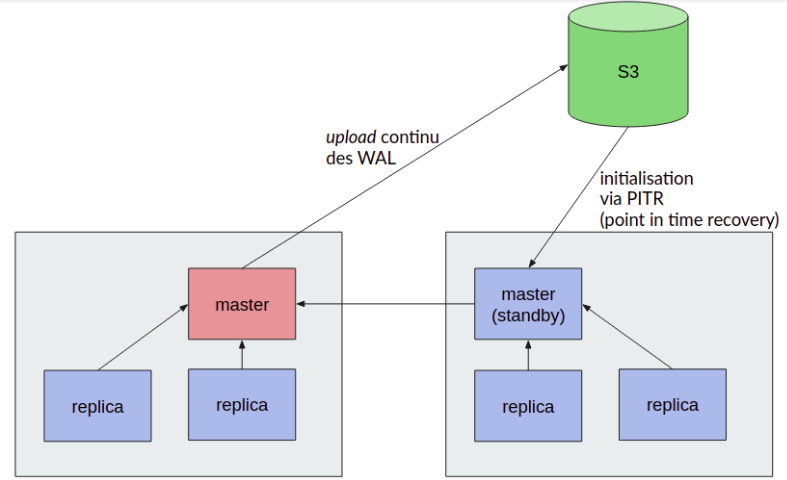
\includegraphics[width=15cm]{images/database-arch}
\end{figure}

Nous avons configurés Stolon pour qu'il déploie une instance de Postgres
par nœud (donc trois par cluster). L'une de ces instance est désignée en
tant que \textit{master} et les autres sont configurées comme étant des
réplicas.

Sur le cluster1, qui est configuré pour ne pas être \textit{master},
l'architecture sera similaire. Cependant la \textit{master} sera mise en
\textit{stand-by} et ne fera que des lectures.

Un cluster de Postgres est initialisé avec l'aide d'un point de
récupération d'un instantané stocké sur notre instance de stockage S3
qui a été envoyé par le \textit{master} de l'instance principale en
envoyant les journaux de transactions (WAL).

\subsection{Sécurisation et analyse des risques}

Seuls l'application web et un micro-service (entrypoint) sont exposés
vers l'extérieur à travers un proxy hébergé à l'AIUS (qui forward
uniquement le trafic TCP des ports 80 et 443 vers les clusters) la
surface d'exposition est minimisée.

L'interface web ainsi que le websocket sont uniquement joignables de
manière sécurisé avec de l'HTTPS.

Cependant n'importe qui depuis le réseau de l'Université ou utilisant le
VPN peut atteindre certains points auxquels ils ne devraient pas avoir
accès. Par exemple, le bus de données que nous utilisons possède un
mécanisme d'authentification pour que seuls les services autorisés
puissent s'y connecter ; hélas par manque de temps cela n'a pas été
configuré et des personnes malintentionnées pourraient y brancher des
services pour écouter ce qui se passe sur le bus et récupérer des
identifiants par exemple.

La machine virtuelle que nous avons à l'AIUS est également un point
critique important : si elle tombe, plus aucun service ne sera
accessible. Le fait d'utiliser \textit{haproxy} de la manière dont on le
fait nous prive de voir l'IP réelle du client depuis les services
hébergés sur les clusters, bien que nous ne nous servons pas, cela
pourrait être utile pour l'analyse de certains logs.

\subsection{Supervision}

La supervision peut s'effectuer à différents niveaux. Tout d'abord il
est possible de récupérer les différentes statistiques du proxy en place
à l'AIUS grâce à l'activation de l'interface web de \textit{haproxy}.

Nous utilisons également un service tiers
(UptimeRobot\footnote{\url{https://uptimerobot.com/}})
pour vérifier si le site est toujours joignable depuis l'extérieur. Le
statut actuel peut être consulté ici : \url{https://status.chatalk.fr/}.

Ce service va effectuer un ping régulier et effectuer régulièrement des
requêtes HTTP vers la page d'accueil et va envoyer un mail à Ludovic en
cas d'incident. L'incident de Renater du 18 décembre 2019 a par exemple
été suivi en temps réel.

Concernant la surveillance au niveau des clusters, nous avons, avec le
projet
\textit{kube-prometheus}\footnote{
  \url{https://github.com/coreos/kube-prometheus}},
déployé une pile de surveillance qui comporte trois éléments
principaux\ :

\begin{itemize}
\item
  Alert Manager, qui permet la configuration d'un certain nombre
  d'alertes,
\item
  Prometheus, qui permet d'afficher ces alertes, de récupérer des
  métriques exposées par Kubernetes ainsi que certaines qui sont
  exposées par certains services en explorant des URL particulières sur
  ces derniers,
\item
  Grafana, qui avec l'aide des métrique récupérées depuis Prometheus, va
  afficher un grand nombre de tableaux de bords avec des graphes, des
  valeurs\ldots{}
\end{itemize}

La figure suivante montre la manière dont tout est connecté ensemble. Le
plan de contrôle de Kubernetes va régulièrement vérifier les services
qui sont configurés pour l'être afin de voir s'ils sont bien
fonctionnels. Prometheus va explorer des URL spécifiées par les services
qui proposent d'exposer leur propres métriques ainsi que celles exposées
par le cluster Kubernetes. Alert Manager va récupérer ces métriques et
voir si certaines d'entre elles dépassent certaines valeurs et va donc
lever certaines alertes. Grafana est une belle interface pour avoir une
vue d'ensemble des métriques récupérées sur Prometheus avec l'aide de
beaux graphes. Les métriques récupérées par Prometheus sont rendues
accessibles au plan de contrôle avec l'aide d'un \textit{Prometheus
Adapter} qui va se charger de rendre les différentes métriques
compréhensibles pour le plan de contrôle. Le plan de contrôle pourra
donc être en mesure de pouvoir augmenter ou diminuer le nombre
d'instances de certains services (utilisation de \textit{Horizontal Pod
Autoscaler}\footnote{
  \url{https://kubernetes.io/docs/tasks/run-application/horizontal-pod-autoscale/}}).

\begin{figure}[h]
  \caption{\label{monitor} La surveillance sous Kubernetes}
  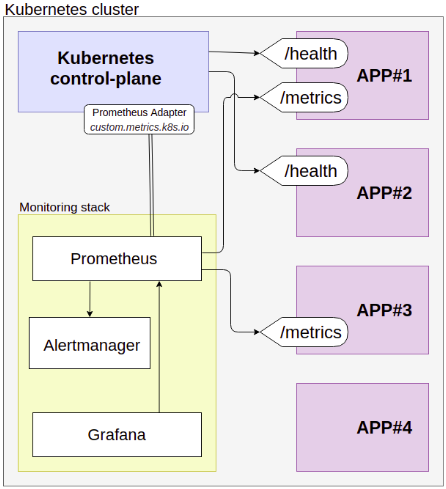
\includegraphics[width=15cm]{images/monitoring}
\end{figure}

En cas de soucis, les logs peuvent être facilement récupérés avec l'aide
de l'outil \textit{kubectl}, qui est un outil en ligne de commandes
utilisé pour gérer un cluster Kubernetes.

\subsection{Double pile v4/v6 + v6-seul}

Nos deux sites ne dispose pas de connectivité IPv6 du fait que
l'Université de Strasbourg n'a pas été en mesure de pouvoir nous en
router. Néanmoins, même avec de l'IPv6 il aurait été compliqué de
configurer convenablement Kubernetes pour prendre en charge la double
pile IPv4/IPv6 qui est encore en stade d'alpha à l'heure actuelle. C'est
donc la raison pour laquelle en interne seul de l'IPv4 est utilisé.

Cependant nous avons fait en sorte que notre application puisse être
accessible pour les utilisateurs que ce soit en IPv4 et en IPv6. Pour ce
faire, Ludovic a déployé un proxy sur une machine virtuelle de l'AIUS,
qui elle est accessible publiquement en IPv4 et en IPv6. Lorsqu'une
connexion d'un utilisateur arrive, le proxy (\textit{haproxy} en
l'occurence), va ouvrir une nouvelle connexion TCP vers les deux sites
en faisant de la répartition de charge sur les clusters disponibles.
